\section{Design}
%
%%%%%%%%%%%%%%%%%%%%%%%%%%%%%%%%%%%%%%%%%%%%%%%%%%%%%%%%%%%
\subsection{Judgments and transcriptions}
%
%%%%%%%%%%%%%%%%%%%%%%%%%%%%%%%%%%%%
\subsubsection{Assumptions}
%
On the one hand, HJ methods have their assumptions rooted in the Classical Test Theory (CTT), where an individual's observed score is composed of a "true score", and a random measurement error. Moreover, the true score is defined as the expected value of the score under an infinite number of independent test administrations\footnote{the National Council of Measurement in Education (NCME) Assessment Glossary: \url{ https://www.ncme.org/resources/glossary}}.

On the other hand, CJ methods hinges on two principles: the law of comparative judgments \citep{Thurstone_1927}, and the consensus of judges \citep{Lesterhuis_2018}. Under the former, the outcome of a comparison, i.e. a relation of preference, is determined by the perceived difference between the discriminal processes of pairs. A \textit{discriminal process}, is the assumed physiological impact that a stimulus has on a listener. However, since this impact cannot be measured directly, we are forced to make some assumption about such process. The minimal assumption we can make is that the process' ordering on the psychological continuum, is the same as the stimulus' ordering that cause them. Moreover, as frequently observed in the field of psycho-physics, since the relationship between stimulus and its impact is not one-to-one, we are also forced to assume the impact has a dispersion/variability, called the \textit{discriminal dispersion}\footnote{for a detailed explanation of the law, see \citet{Thurstone_1927} and \citet{Verhavert_2018} (p. 22-29)}. Finally, the latter principle indicates the shared consensus across judges adds to the validity of the method \citep{Lesterhuis_2018}. This claim is supported by the fact that different listeners differ in the focus and broadness of their judgments \citep{Lesterhuis_2018}, and that each representation is assessed by multiple judges, implying the final score is a reflection of the judges’ collective expertise \citep{Pollitt_2012b}. This only means that by combining various judgments, we come closer to the "true" rankings of SI \citep{Lee_et_al_2014}.
%
%
%%%%%%%%%%%%%%%%%%%%%%%%%%%%%%%%%%%%
\subsubsection{Procedures} \label{ss_sect:proc}
%
The HJ procedure consisted on two psycho-linguistic\footnote{science concerned with human language production, comprehension, and acquisition \citep{Levelt_1993}.} stages: (1) select and mentally represent the stimulus' information, independent of other stimuli\footnote{assumption that is not usually met due to anchoring bias (see section \ref{ss_sect:expset}).}, and (2) rate the representation, according to a task. Therefore, under this procedure, listeners rate the stimulus' SI in an absolute manner, with an 100-point scale going from "very unintelligible" ($0$) to "very intelligible" ($100$) \citep{Boonen_et_al_2021, Faes_et_al_2021}.

In contrast, CJ is composed of three interrelated psycho-linguistic stages: (1) select and mentally represent the information of the pairs, (2) compare and weigh their relevant information, and (3) rate which representation is preferred, according to a task \citep{vanDaal_2020}. As a result, in CJ-D, the listeners rate a pair of stimuli in a dichotomous way, i.e. if stimulus A is more intelligible than B you observe a one in the outcome variable, and zero otherwise \citep{Bradley_et_al_1952}. On the other hand, under CJ-O, the listeners rate both stimuli on a 5-point ordinal scale\footnote{evidence on the quality, reliability, and validity benefits of a 5-point scale can be found in \citet{Revilla_et_al_2014}.} where the outcome variable maps to the following preference relationships: $A>>B$, $A>B$, $A=B$, $A<B$, $A<<B$, where $>>$, $>$, $<<$, $<$, and $=$ symbols indicate the level of preference and indifference between the pairs, respectively \citep{Tutz_1986, Agresti_1992}.
%
%
%%%%%%%%%%%%%%%%%%%%%%%%%%%%%%%%%%%%
\subsubsection{Experimental settings} \label{ss_sect:expset}
%
On both procedures, the experimental settings for the \textbf{judgment task} followed the next steps \citep{Boonen_et_al_2020, Boonen_et_al_2021}:
%
\begin{enumerate} \itemsep1pt
	\item the listener take a seat in front of a computer screen, located at his(her) home, workplace, or the experimental laboratory.
	%
	\item the listener open Comproved\footnote{software developed by the University of Antwerp designed to perform comparative judgments: \url{https://comproved.com/en/a}.} and select the rating task.
	%
	\item the listener read two set of instructions presented on the computer screen about:
	\begin{enumerate}
		\item how to perform the task, and
		\item the aspects not to consider for the task.
	\end{enumerate}
	%
	\item the listener hear the stimuli through high quality headphones, set at a comfortable volume.
	%
	\item the listener rate which stimulus sounded more intelligible by selecting the appropriate button, for CJ-D and CJ-O tasks, or a score from a slider on the computer screen, for the HJ task.
	%
	\item \textcolor{blue}{the listener provide a decision statement on why the selected stimulus sounded more intelligible.}
\end{enumerate}
%
\begin{figure}[h]
	\centering
	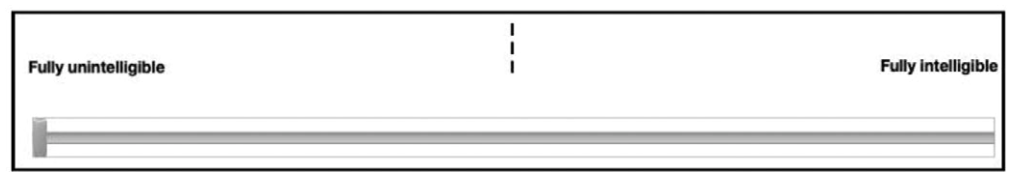
\includegraphics[width=0.8\linewidth]{slider.png}
	%
	\caption[Slider for the HJ task.]%
	{Slider for the HJ task. Extracted from \citet{Boonen_et_al_2021}.}
	\label{fig:slider}
\end{figure}
%
Observational evidence indicate the HJ procedure might suffer from anchoring effects\footnote{a bias in decision that occurs when people anchor their decisions around a reference point, and adjust their choices relative to it \cite{Baddeley_2017, Kahneman_2013}.} or issues with the default option of the slider. About the former, the anchoring seem to happen when listeners consider the previous assessment as a reference point for the next, effectively turning the task into a comparative rating, similar to CJ. About the latter, as the default setting for the slider is located on the far left for each new assessment (as seen in Figure \ref{fig:slider}), it is likely that such setting might impact the rating procedure\footnote{compelling evidence on how default settings impact several decision process can be found in \citet{Kahneman_2013} and \citet{Johnson_et_al_2003}.}. Considering the previous, in order to minimize both issues, care is taken to randomize the display of stimuli within each listener. However, the researcher recognizes that a better approach to face the second problem would be to randomize the default setting of the slider, but this will not be applied nor investigated on the current research. 

\textcolor{red}{talk about decision statements or thinking-at-loud tasks.}

Finally, for the \textbf{transcription task}, the followed steps were similar to the previous task. Although, at the fourth step, the listeners did not rated the stimulus but rather wrote their orthographic transcriptions, in a free text field in the Comproved environment.
%
%
%%%%%%%%%%%%%%%%%%%%%%%%%%%%%%%%%%%%%%%%%%%%%%%%%%%%%%%%%%%
\subsection{Children} \label{s_sect:children}
%
\textcolor{blue}{Thirty three ($33$)} $7$-year old children are selected using a large corpus of \textit{spontaneously spoken speech}, collected by CLiPS over the last twenty years. The selection followed a two step procedure, similar to one outlined in \citet{Faes_et_al_2021}. First, a \textcolor{blue}{convenient sample} of hearing impaired children is selected. Second, a \textcolor{blue}{matched sample} of normal hearing children is selected.

For the first step, a \textcolor{blue}{convenient sample} of \textcolor{blue}{$11$} hearing impaired children with cochlear implant (HI/CI), and \textcolor{blue}{$11$} hearing impaired children with hearing aids (HI/HA) is selected. The selection is based on the quality of their registered stimuli (utterances), as it is defined as in Section \ref{s_sect:stimuli}.

For the second step, \textcolor{blue}{$11$} normal hearing children (NH) are matched on gender, age, and regional background, to the groups selected in the previous step. The matching is done through a \textcolor{blue}{Manual or Propensity Score Matching (PSM)} procedure, \textcolor{red}{explain the appropriate procedure}.

Finally, the researcher considers important to highlight two relevant points from the children's selection process. First, while the matching procedure for the NH group uses the child's \textit{age} (at recording), the method cannot use the same variable for the other two groups. This is due to the fact that \textit{age} is merely used as a proxy, for the amount of time a child has been developing his(her) language. In that sense, a more appropriate variable to use under the HI/CI and HI/HA groups would be e.g. the \textit{device length of use}, which approximates the "hearing age" of such children, or their \textit{vocabulary size}, which resembles their "lexical age" \citep{Faes_et_al_2021}. For this research, we consider the \textit{device length of use} as the simplest one to implement. Second, due to the nature of the sample selection procedure, we cannot ensure the HI/CI and HI/HA, nor the NH group, are representative of their respective populations. Therefore, inferences beyond this particular set of children must be taken with care.

\begin{comment}
%%%%%%%%%%%%%%%%%%%%%%%%%%%%%%%%%%%%
\textbf{for the experimenter:} Based on \citet{Faes_et_al_2021} we depict the procedure for the experimenter:
%
\begin{enumerate}
	\item 1. matching procedure 
	\item selection of suitable stimuli
	\item determine the number of stimuli per judge 
	\item 
\end{enumerate}	
\end{comment}
%
%
%%%%%%%%%%%%%%%%%%%%%%%%%%%%%%%%%%%%%%%%%%%%%%%%%%%%%%%%%%%
\subsection{Stimuli} \label{s_sect:stimuli}
%
The stimuli consisted of the children's utterances (sentences of similar length) recovered from previously mentioned CLiPS corpus. More specifically, we use a portion of the corpus that consisted of $10$ utterances recordings, for each of the \textcolor{blue}{$33$} selected children. The stimuli were documented when the child was telling a story cued by the picture book "Frog, where are you" \citep{Mayer_1969} to a caregiver "who does not know the story". The quality of the stimuli was ensured by selecting utterances with no syntactically ill-formed or incomplete sentences, any background noise, cross-talk, long hesitations, revisions or non-words \citep{Boonen_et_al_2021}. 

As a result, the data set consisted in a total of $320$ utterances\footnote{under the Design of Experiments (DoE) literature, we would say we have $32$ experimental units with $10$ replicate runs each, making a total of $320$ experimental runs. As it is defined in \citet{Lawson_2015}, an experimental unit is the item under study upon which something is changed, while a replicate run is the experiment conducted with the same factor settings, but using different experimental units.} presented to the listeners in a random order, based on the adaptive pairing algorithm \citep{Pollitt_2012b} implemented in Comproved\footnote{evidence suggest that the number of comparisons and pairing algorithm impacts the reliability, validity and efficiency of the procedure \citep{Bramley_2015, Bramley_et_al_2018, Lesterhuis_2018, Verhavert_et_al_2019}. However, this is not investigated in the current research.}.

Similar designs were used by \citet{Boonen_et_al_2020} and \citet{Faes_et_al_2021}. However, in the former case the number of samples were low, while in the latter, the design was unbalanced and not conducive to appropriate inferences from the pairwise comparisons.
%
%
%%%%%%%%%%%%%%%%%%%%%%%%%%%%%%%%%%%%%%%%%%%%%%%%%%%%%%%%%%%
\subsection{Comparisons / assessments}
%
In terms the number of comparison per representation (stimulus) required for CJ, \citet{Verhavert_2018} provided compelling evidence that between $17$ and $20$ comparisons were enough to achieved a reliable score, measured by the Scale Separation Reliability ($SSR=0.80$). The current research uses the higher end of such values ($20$). 

On the other hand, based on \textcolor{red}{[source]} only $5$ assessments per representation were required under the HJ method, \textcolor{red}{to achieve what?}. Therefore, we use the same number of assessments under HJ\footnote{under DoE literature, this implies we will have $20$ and $5$ duplicates for each replicate run, under the CJ and HJ procedures, respectively. As defined in \citet{Lawson_2015}, duplicates are repeated measurements of the same experimental unit from one run, where it is possible the measured dependent variable vary among duplicates due to measurement error.}.
%
%
%%%%%%%%%%%%%%%%%%%%%%%%%%%%%%%%%%%%%%%%%%%%%%%%%%%%%%%%%%%
\subsection{Judges and transcribers} \label{s_sect:JandT}
%
The generation of the ratings required the participation of $180$ judges (listeners). The judges were students from the Toegepaste Taalkunde bachelor or from the Taal- en Letterkunde master's degree. On both cases, the judges participated in the procedure as part of their course credit. \textcolor{blue}{Since we expected the CJ tasks to be 4-times more demanding, in terms of time and effort, than the HJ task, we decided to allocate 4-times more judges to such task}. Table \ref{tab:allocation} describes the judge allocation, the total number of judgments, and the number of judgments per judge.
%
\begin{table}[h!]
	\centering
	\begin{tabular}{|| c c | c | c c| c | c | c || } 
		\hline
		& & Number & \multicolumn{2}{c |}{Number (per stimuli)} & Total & Number & Judgments \\ [0.5ex]
		\cline{4-5}
		& Method & Utterances &  assessments & comparisons & judgments & judges & per judge \\ [0.5ex] 
		\hline\hline
		1 & CJ-D & 320 & n.a. & 20 & 6400 & 80 & 80 \\ 
		2 & CJ-O & 320 & n.a. & 20 & 6400 & 80 & 80 \\
		3 & HJ & 320 & 5 & n.a. & 1600 & 20 & 80 \\
		\hline
		\multicolumn{4}{l}{\footnotesize{n.a.= not applicable}}
	\end{tabular}
	\caption{Design to rate $320$ stimuli per SR method.}
	\label{tab:allocation}
\end{table}
%

On the other hand, for the transcription task, $100$ transcribers participated in the experiment. The participants and stimuli were divided into five groups, where each group of $20$ students ($100/5$) transcribed $64$ stimuli on their series ($320/5$), resulting in $20$ transcriptions per utterance ($64 \times 100 / 320$). In total we registered $6400$ transcriptions\footnoteref{foot:doe}}.
%
%